\documentclass[11pt,UTF8]{ctexart}
\title{单个圆形固体颗粒悬浮流体}
\author{马坤}
\date{2019.11.5}
\usepackage{amsmath}
\usepackage{graphicx}
\usepackage{caption}
\usepackage{subcaption}
\usepackage[left=1in, right=1in, top=1in, bottom=1in]{geometry}
\begin{document}
    \maketitle
    在这个情况下,圆形固体颗粒的圆心处于泊肃叶流体(流体以峰值速
    度为$U_0=0.1$流动)模拟区域的中央;其半径为$r=H/4$,$H=1$是模
    拟区域的宽度,模拟区域的长度为$L=H=1$;流体与颗粒的密
    度都假设为$\rho=1$;此次模拟中我们假设$W=0.1$。我们
    的$\phi$形式如下:
    $$
    \phi=0.5[-\tanh{\frac{2.4(r-1/4)}{W}}+1], r=\sqrt{(x-L/2)^2+(y-H/2)^2}.\eqno(1)
    $$
    \par{$\phi$应该是一个二元函数,图1.a为其三维图片,图1.b为$\phi$在$x=0.5$或者$y=0.5$
    处的投影。在给出的数值的情况下,$\phi$在固体颗粒里面$(r < H/4)$
    为1,在固体外面的液体里面$(r > H/4)$为0,固液交界面$(r = H/4)$为0.5。}
    \begin{figure}[b]
        \centering
        \begin{subfigure}[t]{0.49\textwidth}
            \centering
            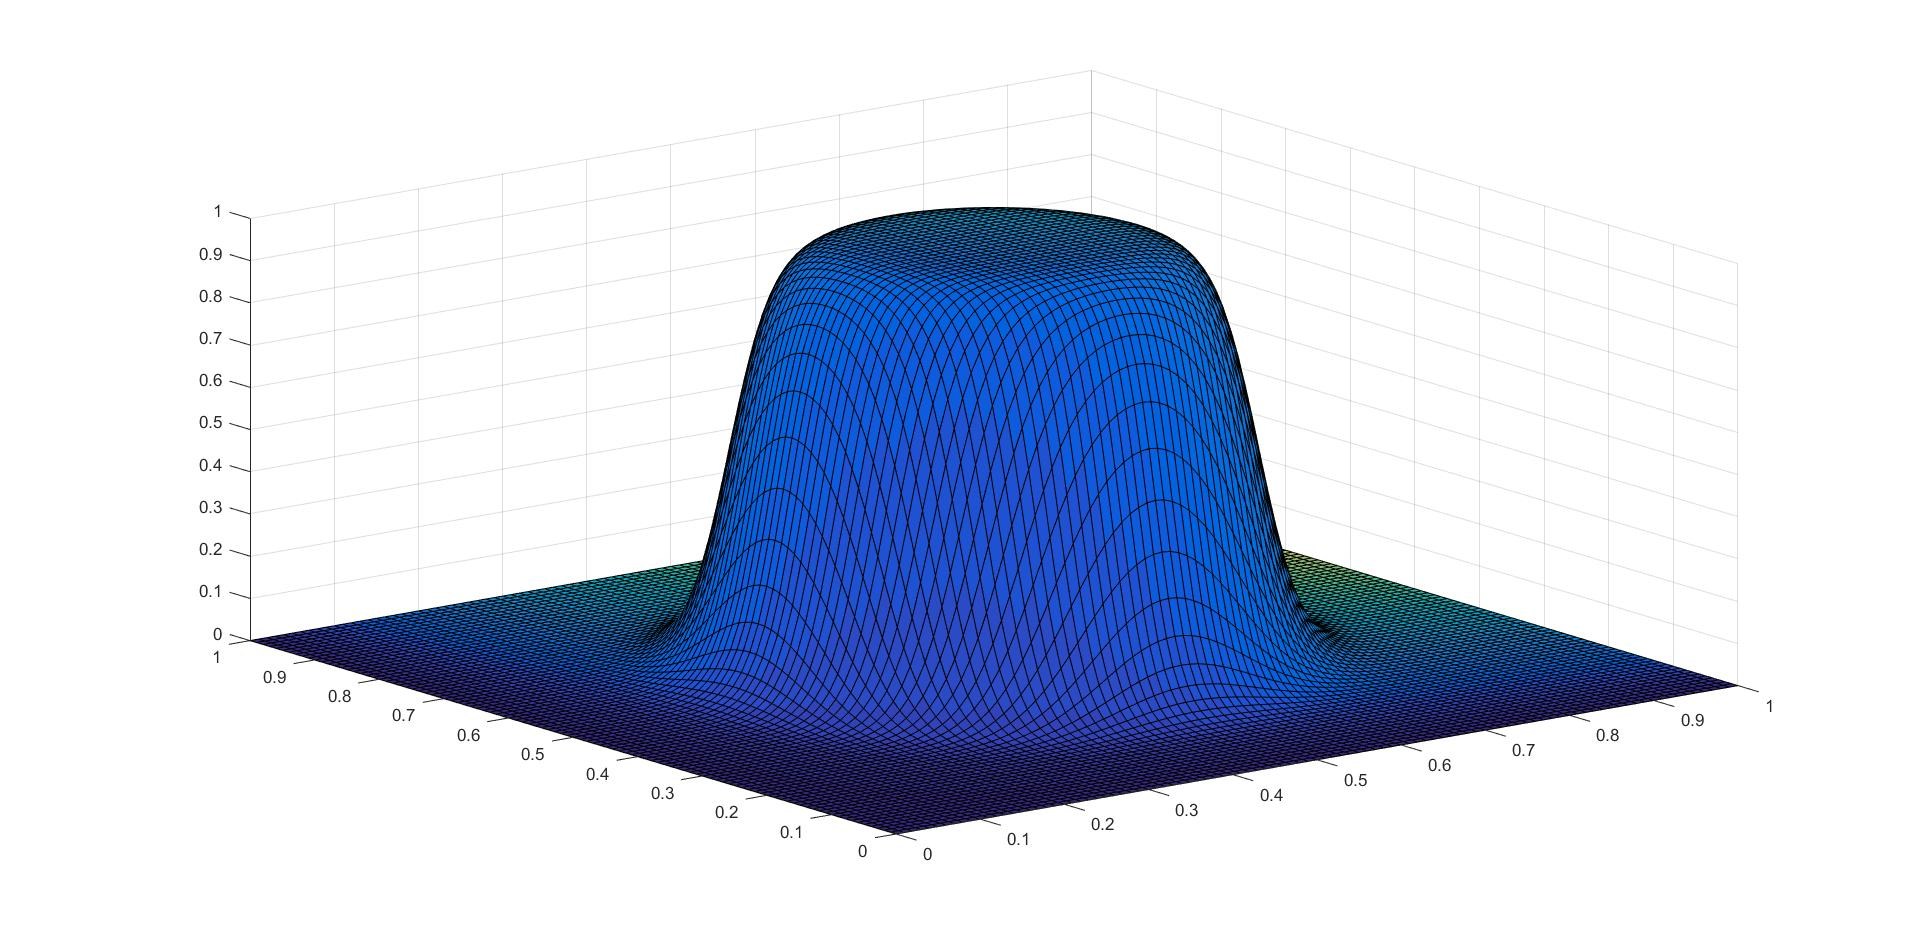
\includegraphics[width=\textwidth]{3D.jpg}
            \caption{$\phi$的3维图片}\label{1.a}
        \end{subfigure}
        \begin{subfigure}[t]{0.49\textwidth}
            \centering
            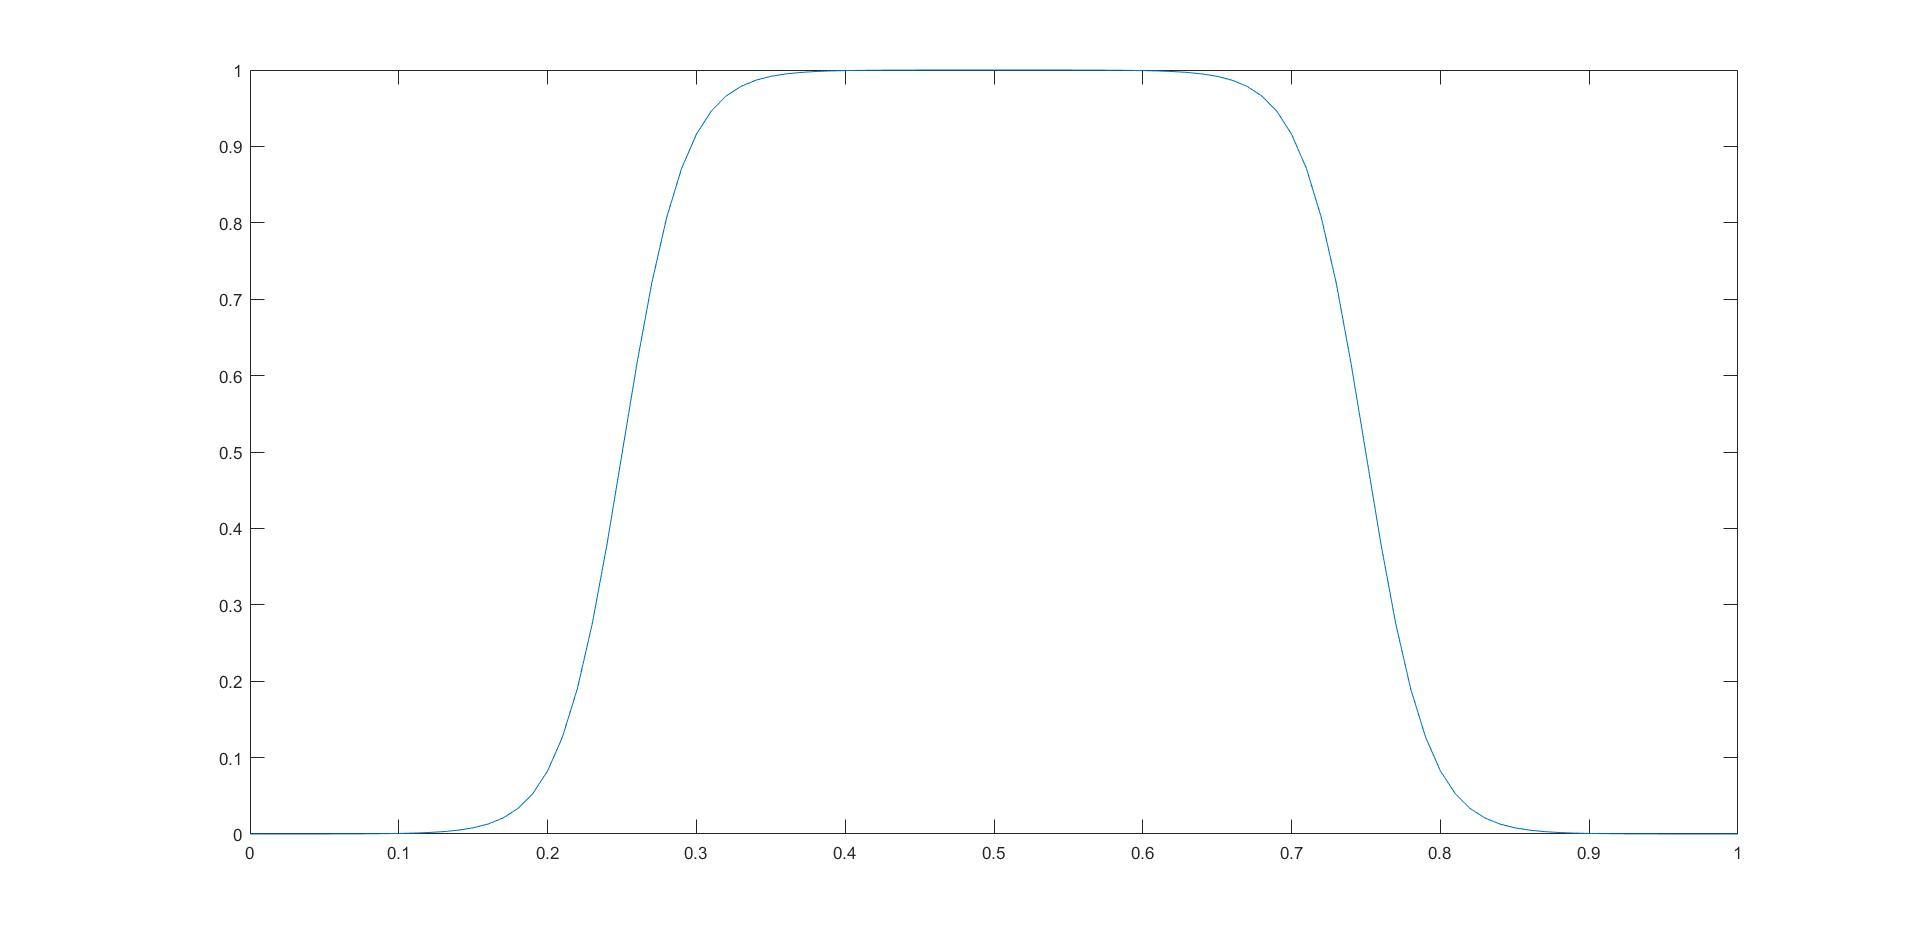
\includegraphics[width=\textwidth]{untitled.jpg}
            \caption{$\phi$在$x=0.5$$(y=0.5)$的投影}\label{1.b}
        \end{subfigure}
        \caption{$\phi$的图像}
    \end{figure}
    \par{模拟中我们假设$\frac{\eta_s}{\eta_l}=50$,我们的粘
    性系数$\eta$有如下表达式:
    $$\eta = 1+\frac{\eta_s}{\eta_l}\phi-\phi.\eqno(2)$$
    可以知道我们的$\eta$的极大值为50,为了和黄老师的论文进行匹配,在数值模拟中
    雷诺数$Re=500$。}
    \par{由于假设的流体与颗粒的密度都假设为$\rho=1$,所以有$\eta
    =\nu$,这会在数值模拟中用到。泊肃叶流的控制方程与解可以写为:}
    $$\nabla p=\nabla\cdot(\eta\nabla u).\eqno(3)$$
    $$u_x=4U_0\frac{y}{H}(1-\frac{y}{H}),u_y=0.\eqno(4)$$
    化简$(3)$得到:
    $$\nabla p=(\nabla u)\nabla \eta  + \eta \triangle u.\eqno(5)$$
    其中
    $$
    \nabla u=\left(
    \begin{array}{cc}
        0 & 4U_0(1-2y)/H \\
        0 & 0
    \end{array}
    \right).\eqno(6)
    $$
    $$\triangle u=\left(
    \begin{aligned}
    -8U_0/H^2 \\
    0
    \end{aligned}
    \right).\eqno(7)
    $$
    $$\nabla \eta=(\frac{\eta_s}{\eta_l}-1)\nabla \phi.\eqno(8)$$
    我们可以利用$\phi,\eta$定义表达式$(1),(2)$计算得到:
    $$\nabla \eta=
        (\frac{\eta_s}{\eta_l}-1)\{-0.5[1-\tanh^2\frac{2.4(r-1/4)}{W}]\frac{2.4}{W}\nabla r\}
    $$
    $$
    where\nabla r=\left(
        \begin{aligned}
            \frac{x-L/2}{\sqrt{(x-L/2)^2+(y-H/2)^2}}    \\
            \frac{y-H/2}{\sqrt{(x-L/2)^2+(y-H/2)^2}}
        \end{aligned}
    \right).\eqno(9)
    $$
    \par{将$(6)(7)(8)(9)$代入$(5)$,得到:
    $$
        \nabla p =\left(
            \begin{array}{cc}
                4U_0(1-2y)(\frac{\eta_s}{\eta_l}-1)
                \{-0.5[1-\tanh^2\frac{2.4(r-1/4)}{W}]\frac{2.4}{W}\frac{y-H/2}{\sqrt{(x-L/2)^2+(y-H/2)^2}}\}/H
                -8\eta U_0/H^2 \\
                0
            \end{array}
            \right).\eqno(10)
    $$
    }
    \par{由于外力与压强有如下关系$F = -\nabla p$,再代入所有实验数值,
    我们可以得到外力的精确表达式,由于压强的$y$方向梯度为0,在$y$方向没有
    力,下面表达式只写$x$方向的力。
    $$
        F =-470.4(y-1/2)^2
        [1-\tanh^2 {24(r-1/4)}]/r
        +0.8(1+24.5[1-\tanh{24(r-1/4)}]).\eqno(11)
    $$
    
    \begin{figure}[h]
        \centering
        \begin{subfigure}[t]{0.49\textwidth}
            \centering
            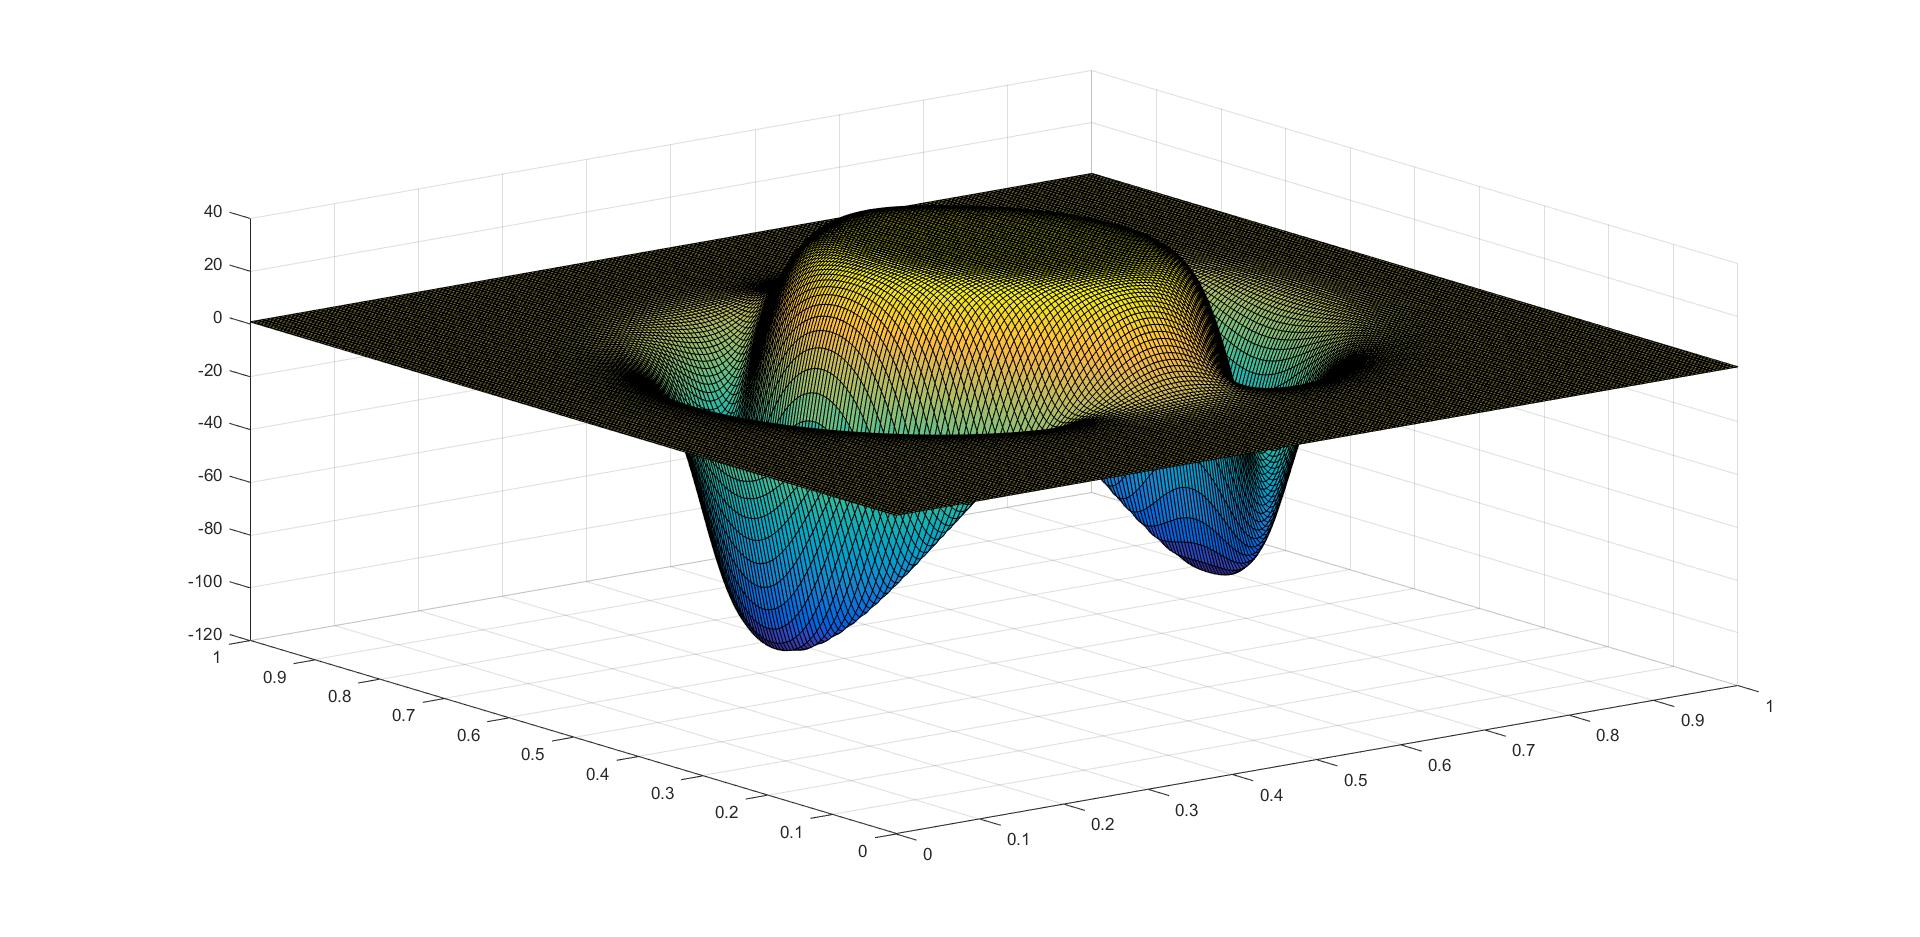
\includegraphics[width=\textwidth]{F3D.jpg}
            \caption{$F$的3维图片}\label{1.a}
        \end{subfigure}
        \begin{subfigure}[t]{0.49\textwidth}
            \centering
            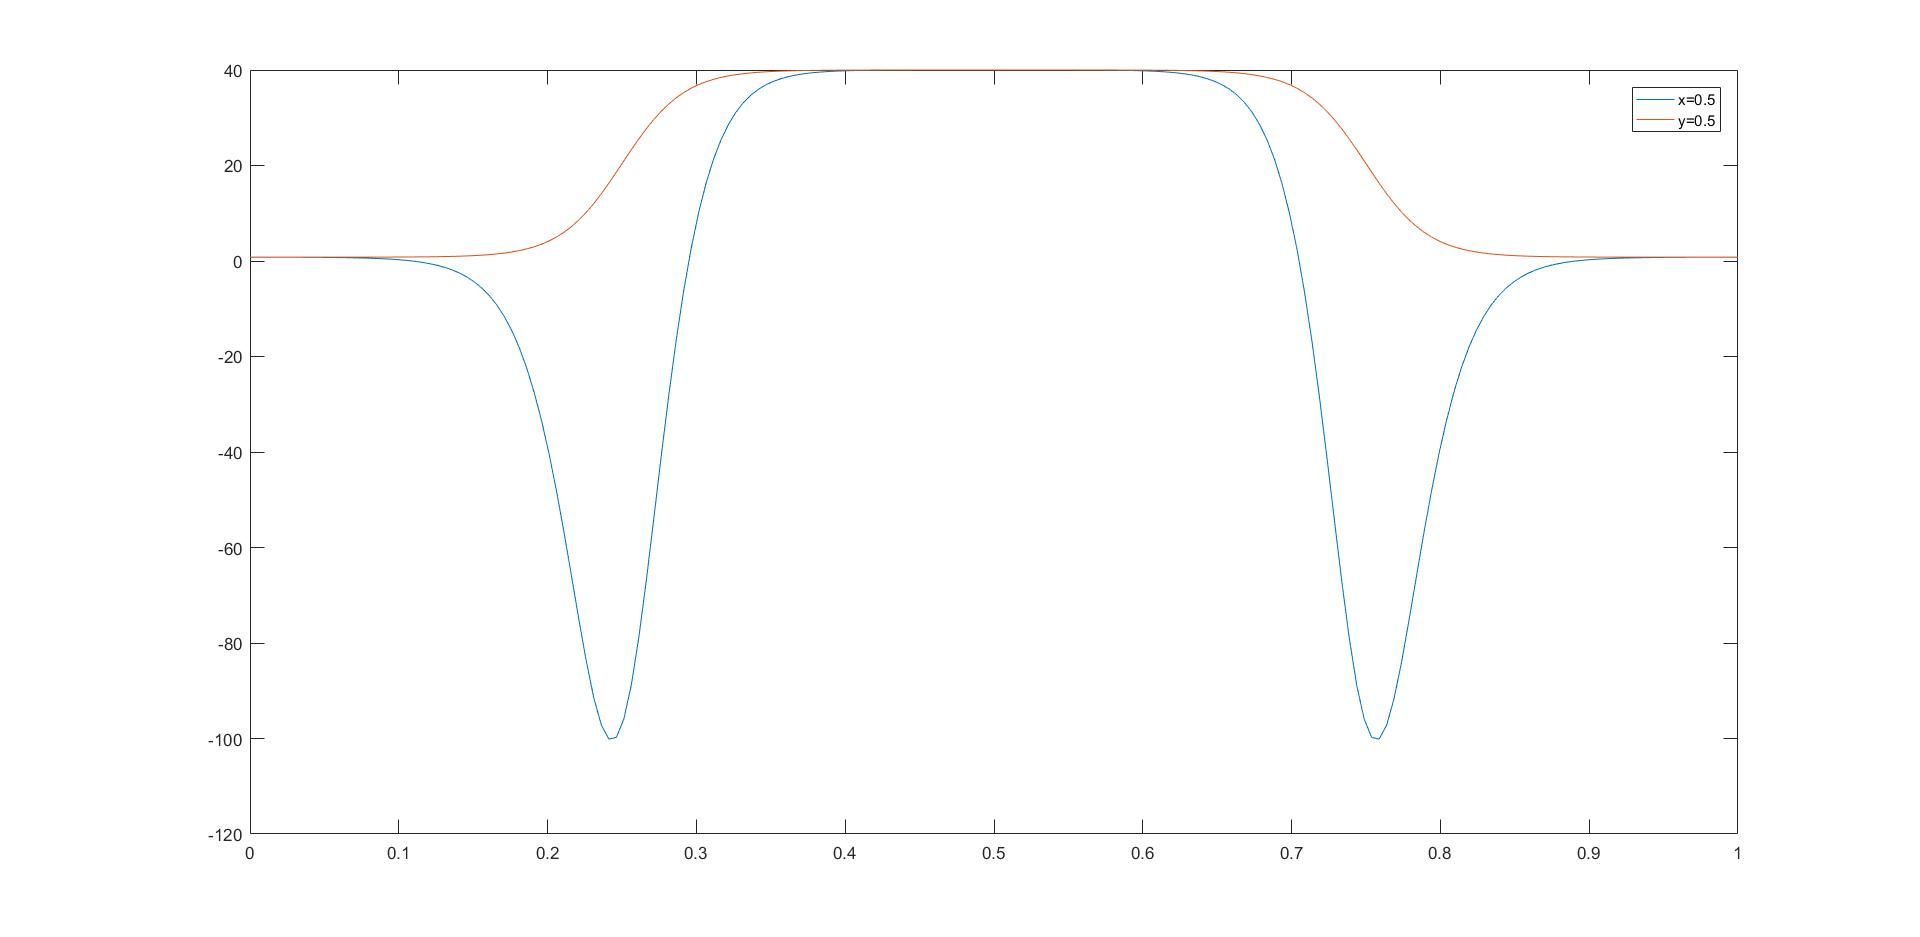
\includegraphics[width=\textwidth]{F2D.jpg}
            \caption{$F$在$x=0.5$$(y=0.5)$的投影}\label{1.b}
        \end{subfigure}
        \caption{$F$的图像}
    \end{figure}
    }
    \par{图2是力在给定的数值下的图像,图2.a为力的三维图像,图2.b为$F$在
    $x=0.5$$(y=0.5)$的投影。可以发现力的最大值为40,最小值为负值,负值
    出现的位置为圆形颗粒的上下边界附近,左右边界没有负值。从图像上来看
    整个系统并不是完全对称的,所以力在上下边界和左右边界有所不同也很正常。}
\end{document}